\subsection{Waveform parameterisation and optimisation}
\label{subsec:pureshift__chirpopt}

Given that a working optimisation setup, including cost functions, had been developed, it was a logical step to then test it out on a more challenging problem: namely, how the waveform used in the PSYCHE PSE could be modified.
This goes beyond simply modifying the number of saltires, as was done in \cref{sec:pureshift__nsaltire}.
There is no real reason why the pulse \textit{must} be an integer number of saltires: in principle it can have \textit{any} shape, although being symmetric about the centre of the pulse would likely still be beneficial in terms of preserving the mechanism of spatiotemporal averaging.

A naive attempt at optimising the pulse would simply involve modifying every pulse point in the double-saltire waveform used in the PSYCHE element.
As described in \cref{sec:theory__rotating_frame}, each pulse point consists of a pair of $x$- and $y$-amplitudes $(c_x, c_y)$; therefore, for a pulse with $m$ points, we would have a parameter vector $\symbf{x} \in \mathbb{R}^{2m}$.
Unfortunately, for PSYCHE, $m$ is on the order of $10000$, and an optimisation with $20000$ points is totally unfeasible.%
\footnote{Although problems of this size have been tackled using optimal control theory\autocite{Khaneja2005JMR,deFouquieres2011JMR,Glaser2015EPJD,Goodwin2016JCP}, it is not really feasible to use it in cases where the pulse is applied \textit{together} with a gradient, as is the case in PSYCHE. On top of that, the coupling networks and spin systems of interest are rather more complicated than in typical applications of optimal control.}

As a result of this, we must consider other ways of parameterising the waveform which use fewer degrees of freedom.
Several approaches to this issue have surfaced in the literature, such as the use of Fourier series\autocite{Geen1991JMR,Kupce1995JMRSB}, Gaussian cascades\autocite{Emsley1990CPL}, or spline interpolation between a subset of pulse points\autocite{Ewing1990CP}.
In this instance, we can use the knowledge that the PSYCHE PSE is composed of saltire pulses to our advantage.
Each saltire pulse is a linear combination of two chirps, defined by:
\begin{align}
    \phi(t) &= \phi_0 + 2\pi f_0 t + \pi\taup(\Delta F)\left(\frac{t}{\taup} - \frac{1}{2}\right)^2 \label{eq:chirp_pulse_phase} \\
    c_x(t) &= A \cos[\phi(t)] \label{eq:chirp_pulse_cx} \\
    c_y(t) &= A \sin[\phi(t)] \label{eq:chirp_pulse_cy}
\end{align}
for $t \in [0, \taup]$. Here, $\taup$ is the duration of the chirp, $A$ is the amplitude of the chirp (which is time-independent), $\phi_0$ the phase of the chirp, $\Delta F$ the bandwidth, and $f_0$ its frequency offset (i.e. where the centre of the bandwidth lies).
The latter two parameters are assumed to be given in units of ordinary frequencies (Hz), not angular frequencies.
(Note that \cref{eq:chirp_pulse_cx,eq:chirp_pulse_cy}, defining the $x$- and $y$-coefficients of the pulse, are just a restatement of \cref{eq:pulse_cartesian}.)

\begin{figure}[htb]
    \centering
    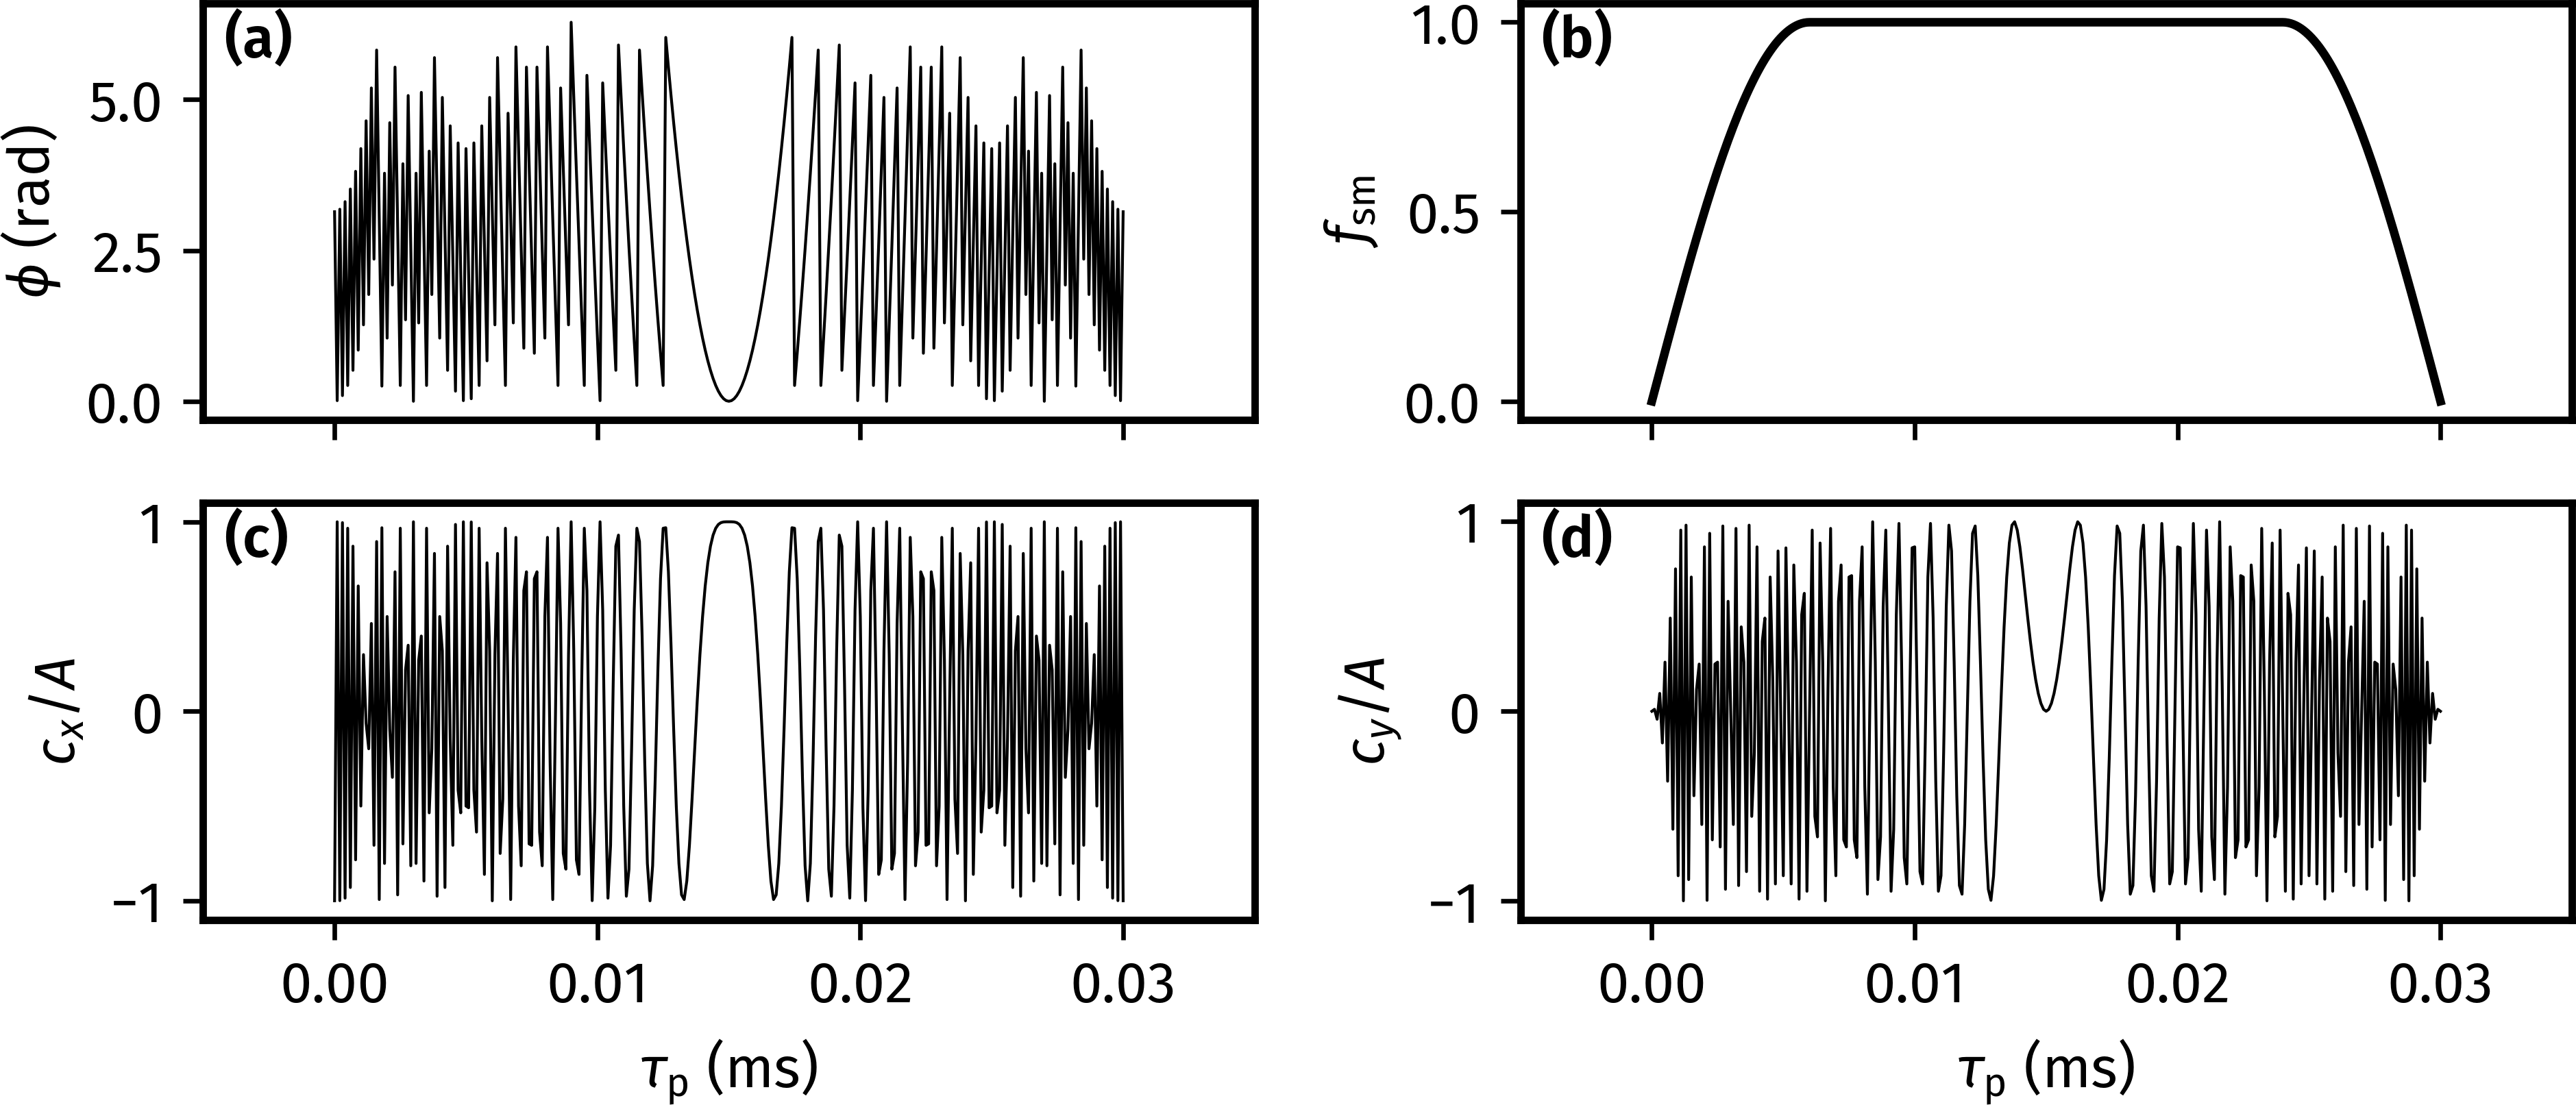
\includegraphics[]{pureshift/chirp_coefficients.png}
    {\phantomsubcaption\label{fig:chirp_coefficients_phase}}
    {\phantomsubcaption\label{fig:chirp_coefficients_smoothing}}
    {\phantomsubcaption\label{fig:chirp_coefficients_cx}}
    {\phantomsubcaption\label{fig:chirp_coefficients_cy}}
    \caption[Phase and Cartesian amplitudes of a typical chirp pulse]{
        Plots of the quantities in \cref{eq:chirp_pulse_phase,eq:chirp_pulse_cx,eq:chirp_pulse_cy} for a typical chirp pulse ($\taup = \SI{30}{\ms}$, $\Delta F = \SI{10}{\kHz}$).
        \textbf{(\subref{fig:chirp_coefficients_phase})} $\phi(t)$ wrapped to the range $[0, 2\pi)$.
        \textbf{(\subref{fig:chirp_coefficients_smoothing})} The quarter-sine smoothing profile which is later applied to the entire waveform (\cref{eq:sming_function}); here $s_\text{sm} = 0.2$.
        \textbf{(\subref{fig:chirp_coefficients_cx})} $c_x(t)/A$ prior to smoothing.
        \textbf{(\subref{fig:chirp_coefficients_cy})} $c_y(t)/A$ prior to smoothing.
        The amplitude $A$ is simply a constant, which is related to the flip angle of the chirp.\autocite{Foroozandeh2018CEJ}
    }
    \label{fig:chirp_coefficients}
\end{figure}

Given these expressions, we see that there are five parameters of the chirp which can be modified: $A$, $\taup$, $\phi_0$, $\Delta F$, and $f_0$.
The two chirps which form one saltire pulse simultaneously sweep in opposite directions, which mean that $\Delta F$ for one chirp is the negative of the other; however, their parameters are otherwise equal.
We may, however, also envision a case where the pulse is constructed from two chirps which are applied at a different point in time.
This adds one more parameter to each chirp, namely $t_0$, the starting time of the pulse)
Each chirp therefore sweeps from the frequency $f_0 - (\Delta F)/2$ at a time $t_0$, to the frequency $f_0 + (\Delta F)/2$ at a time $t_0 + \taup$.
In total, this gives us 12 parameters to optimise.

After constructing the sum of two chirps, `empty' regions of no RF application ($c_x = c_y = 0$) at the beginning and the end were trimmed off.
Since a sum of two chirps is not necessarily symmetric (with respect to reflection in time), the waveform was then reflected about its end, thus doubling the length of the pulse.
The entire waveform was then multiplied by a \textit{smoothing function} $f_\text{sm}(t)$ (\cref{fig:chirp_coefficients_smoothing}), which prevents large jumps in RF amplitude at the beginning and end of the pulse.
$f_\text{sm}$ depends on a smoothing parameter $s_\text{sm}$, which is typically $0.1$--$0.2$:
\begin{equation}
    \label{eq:sming_function}
    f_\text{sm}(t) = \begin{cases}
        \displaystyle \sin\left(\frac{\pi t'}{2 s_\text{sm}}\right) & 0 \leq t' < s_\text{sm}; \\
        \displaystyle 1 & s_\text{sm} \leq t' < 1 - s_\text{sm}; \\
        \displaystyle \sin\left[\frac{\pi (1 - t')}{2 s_\text{sm}}\right] & s_\text{sm} \leq t' \leq 1, \\
    \end{cases}
\end{equation}
where $t' = t/\taup$ (and here $\taup$ refers to the duration of the \textit{entire} waveform, after reflection.).

The initial point chosen was:
\begin{itemize}
    \item Chirp 1: $\taup = \SI{15}{\ms}$; $\Delta F = \SI{-5}{\kHz}$; $\phi_0 = 0$; $A = \SI{36}{\Hz}$; $t_0 = 0$; $f_0 = \SI{5}{\kHz}$;
    \item Chirp 2: $\taup = \SI{15}{\ms}$; $\Delta F = \SI{5}{\kHz}$; $\phi_0 = 0$; $A = \SI{36}{\Hz}$; $t_0 = 0$; $f_0 = \SI{-5}{\kHz}$.
\end{itemize}
After the sum of these two pulses is reflected about its end, we obtain a single saltire with bandwidth \SI{10}{\kHz}, duration $\SI{30}{\ms}$, and an amplitude of $\SI{72}{\Hz}$, corresponding to a flip angle of approximately \ang{32}.

\begin{figure}[htbp]
    \centering
    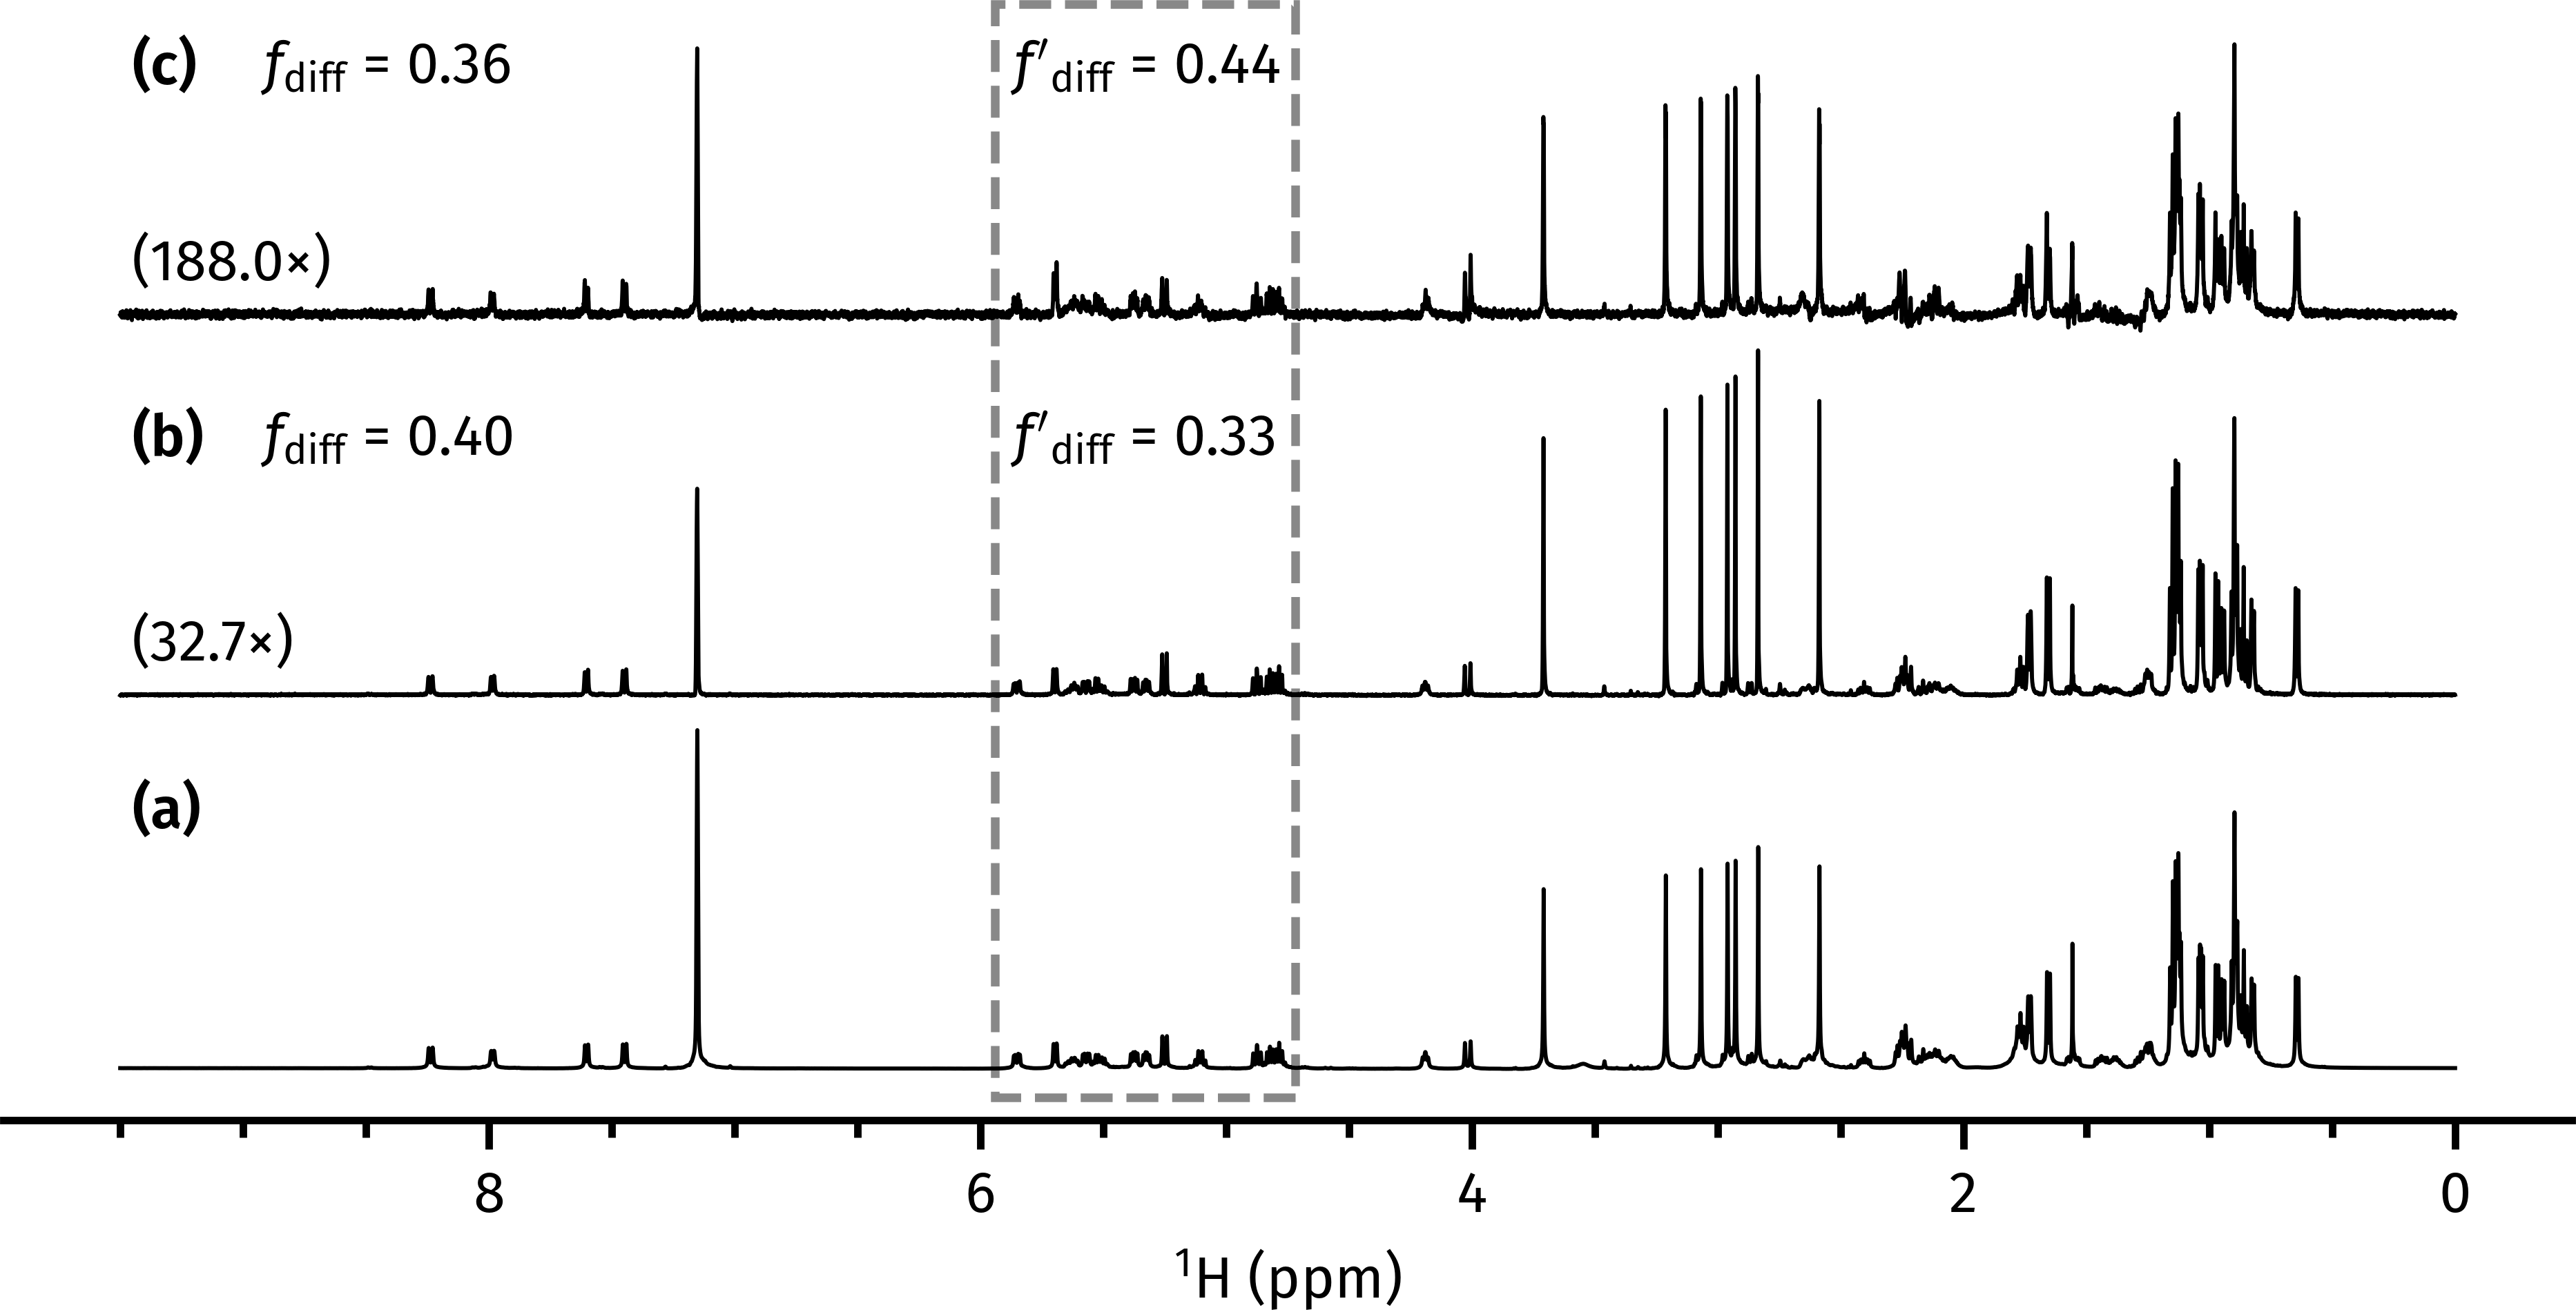
\includegraphics[]{pureshift/chirpopt_spurious.png}
    {\phantomsubcaption\label{fig:chirpopt_spurious_target}}
    {\phantomsubcaption\label{fig:chirpopt_spurious_saltire}}
    {\phantomsubcaption\label{fig:chirpopt_spurious_badoptimum}}
    \caption[Spurious optimum obtained in waveform optimisation using $f_\text{diff}$]{
        \textbf{(\subref{fig:chirpopt_spurious_target})} Target spectrum (pulse--acquire).
        \textbf{(\subref{fig:chirpopt_spurious_saltire})} JRSE spectrum obtained using the initial guess (a saltire).
        \textbf{(\subref{fig:chirpopt_spurious_badoptimum})} JRSE spectrum obtained with a spurious optimum point.
        The grey dotted box shows the restricted region over which $f_\text{diff}$ was subsequently applied to, yielding a formally different cost function $f'_\text{diff}$; this yielded more sensible results where the cost function for the saltire pulse was smaller.
        \datacode{6C-190823}
    }
    \label{fig:chirpopt_spurious}
\end{figure}

Using this setup, several optimisations of the 12 parameters above were conducted using the $f_\text{diff}$ cost function, which had performed well enough in the flip angle optimisations.
However, it was quickly noticed that this led to spurious optima being located, such as the one in \cref{fig:chirpopt_spurious_badoptimum}.
Although the initial point (a saltire) yielded a much larger SNR (\cref{fig:chirpopt_spurious_saltire}), the value of $f_\text{diff}$ was still larger (i.e.\ worse) than for this false optimum.
The reason for this is almost certainly because the saltire pulse distorts the relative intensity of the strong singlets in the spectrum, notably the $\ch{C6D5H}$ peak at \SI{7.15}{ppm}, and the \textit{N}-methyl groups between 2.5 and \SI{3.8}{\ppm}), whereas the false optimum does not (most likely by coincidence).

Of course, singlets are completely unimportant when devising a pure shift experiment.
Unfortunately, singlets are also typically more intense than the rest of the spectrum, and thus contribute disproportionately to the cost function.
A simple and effective way to circumvent this is to restrict the region of the spectrum being evaluated.
In this case, I chose to use the cyclosporin $\ch{H}^{\alpha}$ region between 4.72 and \SI{5.94}{ppm} (grey dotted box in \cref{fig:chirpopt_spurious}).
This yields a formally different cost function, which I label as $f'_\text{diff}$.
With this, much more logical behaviour was observed: in particular, the saltire pulse performed better than the spurious optimum previously found.

While this new cost function could be successfully used to run optimisations, most of these unfortunately failed to find anything performing better than the original saltire pulse.
On the rare occasion where something `better' was found (as judged by the new cost function $f'_\text{diff}$), these `optimised' pulses were fairly close to a saltire, and the corresponding decreases in the cost function extremely small---suggesting that the `better' result may simply just have been due to noise in the cost function.
Nevertheless, these new `optima' \textit{did} function as perfectly serviceable PSEs: for example, \cref{fig:newpulse_tsepsyche} compares a \ac{tse} PSYCHE spectrum obtained with an `optimised' pulse to one obtained with the single saltire pulse.
There is virtually no difference.
This is a meaningful result, as it demonstrates that $f'_\text{diff}$ is actually an accurate metric to determine the quality of a PSE (it is noisy, but this is to be expected of an experimentally measured cost function).
Unfortunately, although the pulse shape is shown in \cref{fig:newpulse_tsepsyche_newpulse}, the exact parameters which led to this pulse shape have been lost to time.

\begin{figure}[htb]
    \centering
    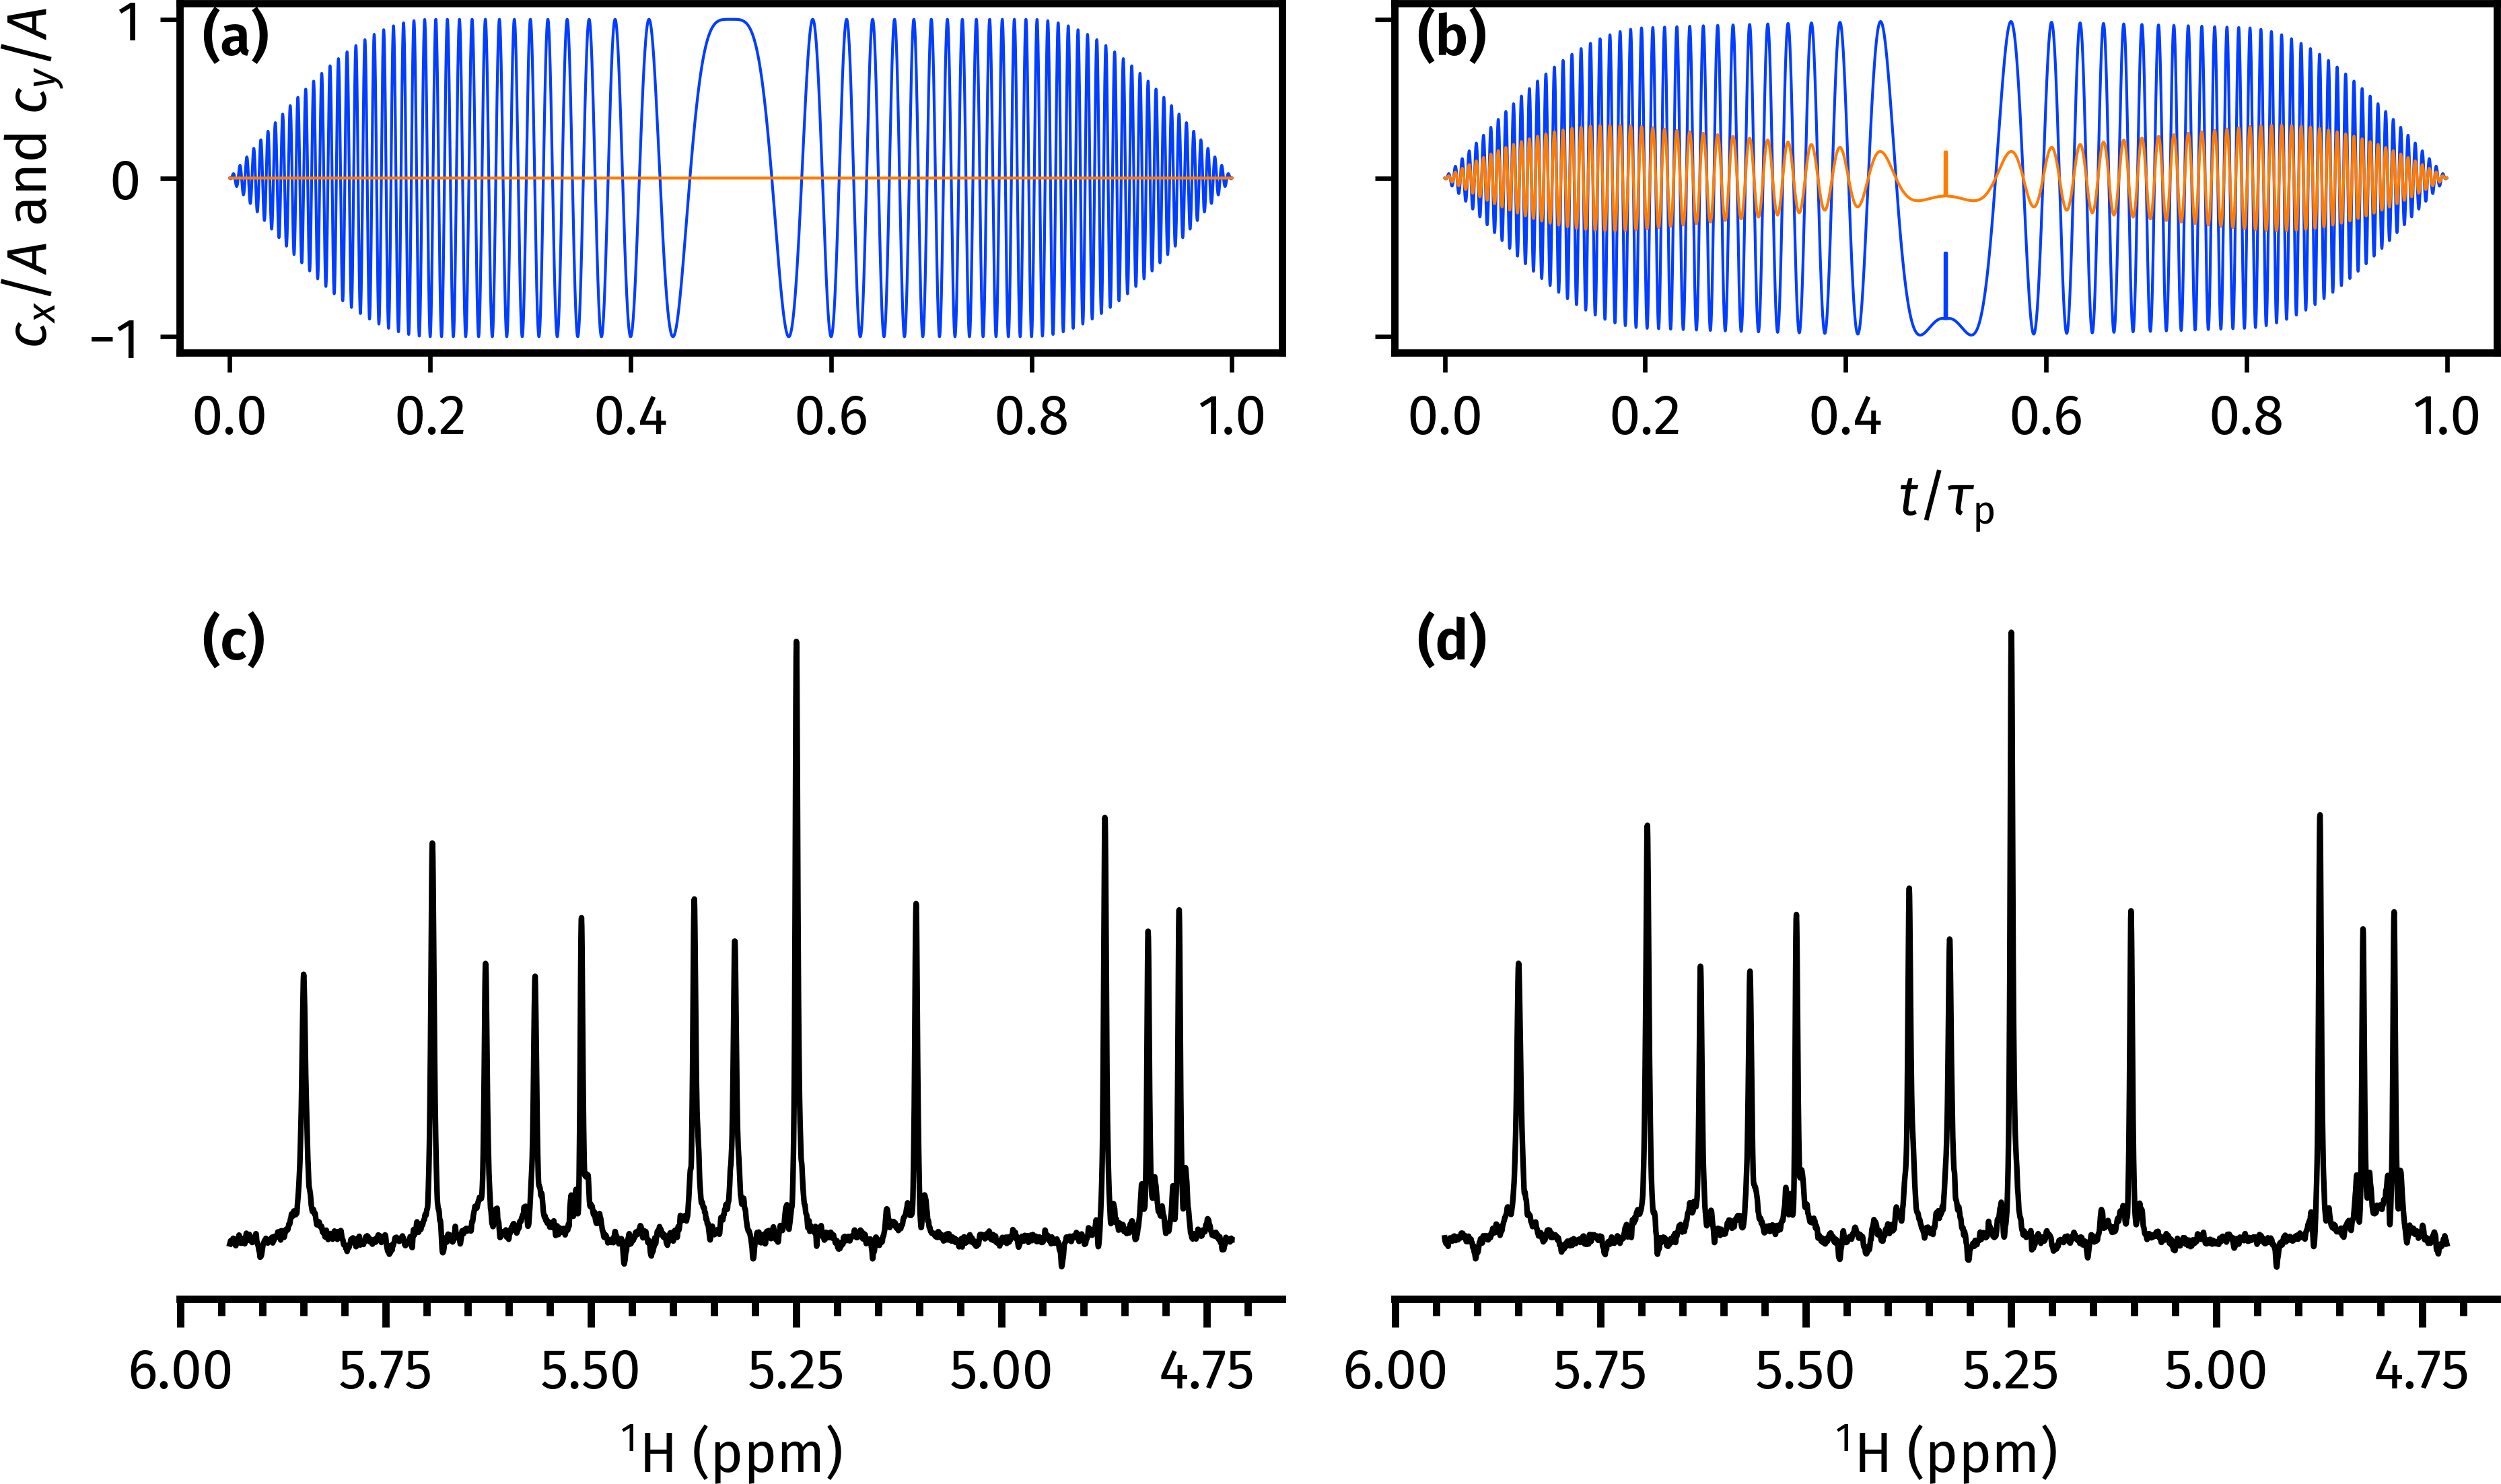
\includegraphics[]{pureshift/newpulse_tsepsyche.png}
    {\phantomsubcaption\label{fig:newpulse_tsepsyche_saltire}}
    {\phantomsubcaption\label{fig:newpulse_tsepsyche_newpulse}}
    {\phantomsubcaption\label{fig:newpulse_tsepsyche_saltirespec}}
    {\phantomsubcaption\label{fig:newpulse_tsepsyche_newpulsespec}}
    \caption[Evaluation of an `optimised' pulse in a TSE-PSYCHE experiment]{
        \textbf{(\subref{fig:newpulse_tsepsyche_saltire})} $x$- and $y$-coefficients of the initial saltire pulse (as a fraction of the maximum amplitude $A$).
        \textbf{(\subref{fig:newpulse_tsepsyche_newpulse})} $x$- and $y$-coefficients of the `optimised' pulse (as a fraction of the maximum amplitude $A$).
        \textbf{(\subref{fig:newpulse_tsepsyche_saltirespec})} TSE-PSYCHE spectrum obtained with the initial guess (a saltire pulse).
        \textbf{(\subref{fig:newpulse_tsepsyche_newpulsespec})} TSE-PSYCHE spectrum obtained with the `optimised' pulse, with virtually equivalent performance.
        \datacode{6C-190831}
    }
    \label{fig:newpulse_tsepsyche}
\end{figure}

One issue is that the optimisation algorithms used here can only perform a \textit{local} optimisation, i.e.\ it may not necessarily locate a global optimum.
We cannot rule out the possibility that \textit{some} pulse within this parameter space may in fact outperform a saltire pulse.
However, finding this optimum---which may lie very far away from the initial guess of a saltire pulse---is not generally something which can be accomplished in a reasonable amount of time, even though 12 parameters is far more tractable than 20000.
Furthermore, the cost functions described here do work, they are generally quite `flat', in that they do not discriminate very sharply between `good' and `bad' spectra.
Combined with the fact that the cost function is noisy, this makes experimental optimisation of the waveform an uphill task.
Nevertheless, much of the knowledge (and code) in this section was later used in the development of POISE.

In the next two sections in this chapter, I move on from PSYCHE and instead discuss completely different methods of obtaining pure shift spectra using only hard pulses in the PSE.
